% опринципиальная схема установки
% общее описание работы приборчиков

Получение ультрахолодного облака атомов Tm происходит в несколько этапов, принципиальная схема приведена на рис.  \ref{fig:expT}.

\begin{figure}[h]
    \centering
    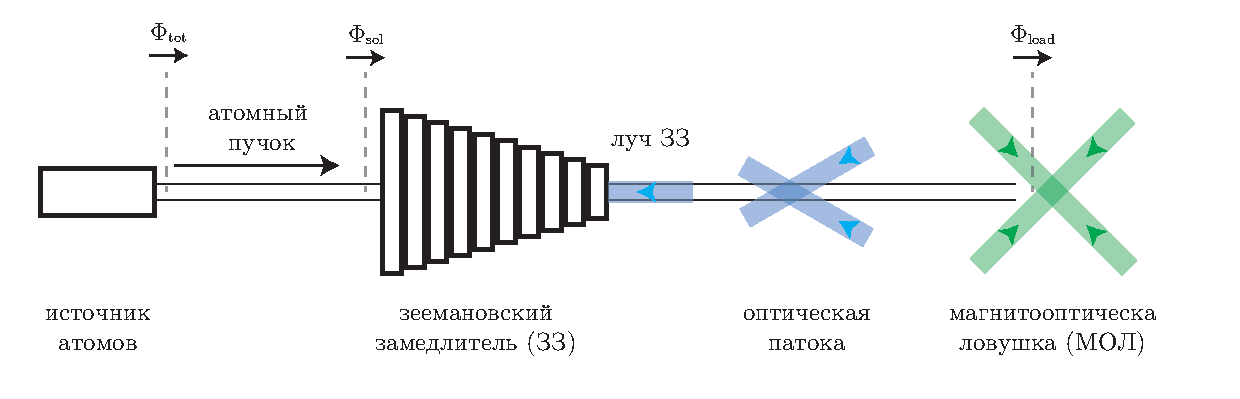
\includegraphics[width=1.0\textwidth]{figs/sheme.pdf}
    \caption{Принципиальная схема установки}
    \label{fig:expT}
\end{figure}


\begin{enumerate}
    \item Источник атомов (печь). Внутри высокого вакуума (ВВ) расположен тигель в печи с кусочком Tm, температура контролируется термопарой. В установке не достигается температура плавления Tm (1545 $\dC$), так что кусочек остаётся в твёрдом состоянии, с его поверхности происходит сублимация атомов, формируя газ атомов Tm с давлением порядка давления насыщенных паров. Поток атомов из печи далее упоминается как $\sub{\Phi}{tot}$.
    \item Атомы вылетают из сопла печи, и попадают в зеемановский замедлитель (ЗЗ). Для охлаждения атомов используется встречный резонансный лазерный пучок на длине волны 410.6 нм и мощности порядка 70 мВт, магнитными катушками создаётся градиент магнитного поля (рис. \ref{fig:zB}) так, чтобы вдоль всей длины ЗЗ атомы выходящие из резонанса из-за доплеровского сдвига, оставались бы в резонансе за счёт зеемановского сдвига.  Поглощая фотоны атомы замедляются, т.к. дальнейшее переизлучение происходит изотропно. 
    \item После прохождения ЗЗ атомы дополнительно тормозятся встречными лучами оптической патоки, для охлаждения используется порядка 15 мВт излучения на длине волны 410.6 нм. С помощью АОМ добивается отстройка от атомного резонанса порядка $1.7\Gamma$. Механизм замедления аналогичен ЗЗ, однако наличие дополнительных охлаждающих встречных пучков перед МОЛ позволяет существенно увеличить скорость захвата системы оптическая патока + МОЛ. 
    \item После оптической патоки происходит захват в МОЛ, на длине волны 530.7 нм, общая потребляемая мощность лазерного излучения порядка 370 мВт, отстройка от резонанса порядка $10\Gamma$. Резонансным лазерным излучением создаётся замедляющая сила, аналогичная вязкому трению, вместе с используемыми в антигельмгольцевской конфигурации катушками, в нуле магнитного поля создаётся минимум потенциала. 
\end{enumerate}
